\documentclass[
	letterpaper, % Paper size, specify a4paper (A4) or letterpaper (US letter)
	10pt, % Default font size, specify 10pt, 11pt or 12pt
]{CSUniSchoolLabReport}

%----------------------------------------------------------------------------------------
%	REPORT INFORMATION
%----------------------------------------------------------------------------------------

\title{Operational Amplifier Circuits, Design, and Limitations \\ Circuits \& Signals \\ EECE2150} % Report title

\author{Michael \textsc{Brodskiy}}

\date{March 23, 2023} % Date of the report

%----------------------------------------------------------------------------------------


\begin{document}

\maketitle % Insert the title, author and date using the information specified above

\begin{center}
	\begin{tabular}{l r}
		Date Performed: & March 15, 2023 \\ % Date the experiment was performed
        Partner: & Juan \textsc{Zapata} \\ % Partner names
		Instructor: & Professor \textsc{Sun} % Instructor/supervisor
	\end{tabular}
\end{center}

\setcounter{section}{-1}

\section{Introduction}

The purpose of this laboratory experimentation is to advance our knowledge of operational amplifiers and their abilities. By applying concepts of the transfer function and fast Fourier transforms, we were able to more thoroughly analyze operational amplifier response.

  \section{Part I}

  \subsection{Q1} The calculations resulted in the following:

  \vspace{5pt}

  \begin{itemize}

    \item The theoretical in-band gain ($|H(\omega)|$): $\dfrac{R_f}{\sqrt{R_s^2 + \dfrac{1}{(\omega C_s)^2}}}=\dfrac{200000}{\sqrt{10^{10}+\dfrac{10^{16}}{\omega^2}}}$

    \item The time constant ($\tau$): $\tau=R_sC_s=(100\cdot10^3)(10\cdot10^{-9})=1[\si{\milli\second}]$

    \item The cutoff angular frequency ($\omega_c$): $\omega_c=\dfrac{1}{\tau}=\frac{1}{.001}=1000\left[ \dfrac{\text{rad}}{\si{\second}} \right]$

    \item The cutoff frequency ($f_c$): $\dfrac{\omega_c}{2\pi}=159.155[\si{\hertz}]$

  \end{itemize}

  \subsection{Q2} The measured gain is $\dfrac{1.11}{.45}=2.467$

  \subsection{Q3} The cutoff frequency does not agree with the theoretical value (it becomes $86[\si{\hertz}]$ instead of 159$[\si{\hertz}]$)

  \begin{figure}[h!]
    \centering
    \includegraphics[width=.9\textwidth]{Figures/L11Osc.png}
    \caption{Oscilloscope Reading of Input and Output}
    \label{fig:1}
  \end{figure}

  \subsection{Q4} That statement is incorrect — The gain increases with higher frequencies.

  \subsection{Q5} The input is square, while the output is like a combined exponential. The output wave looks as it does because, when the square wave is positive or negative, the capacitor is charging. In between, the capacitor voltage jumps to infinity as it shifts.

  \begin{figure}[h!]
    \centering
    \tikzset{every picture/.style={line width=0.75pt}} %set default line width to 0.75pt        

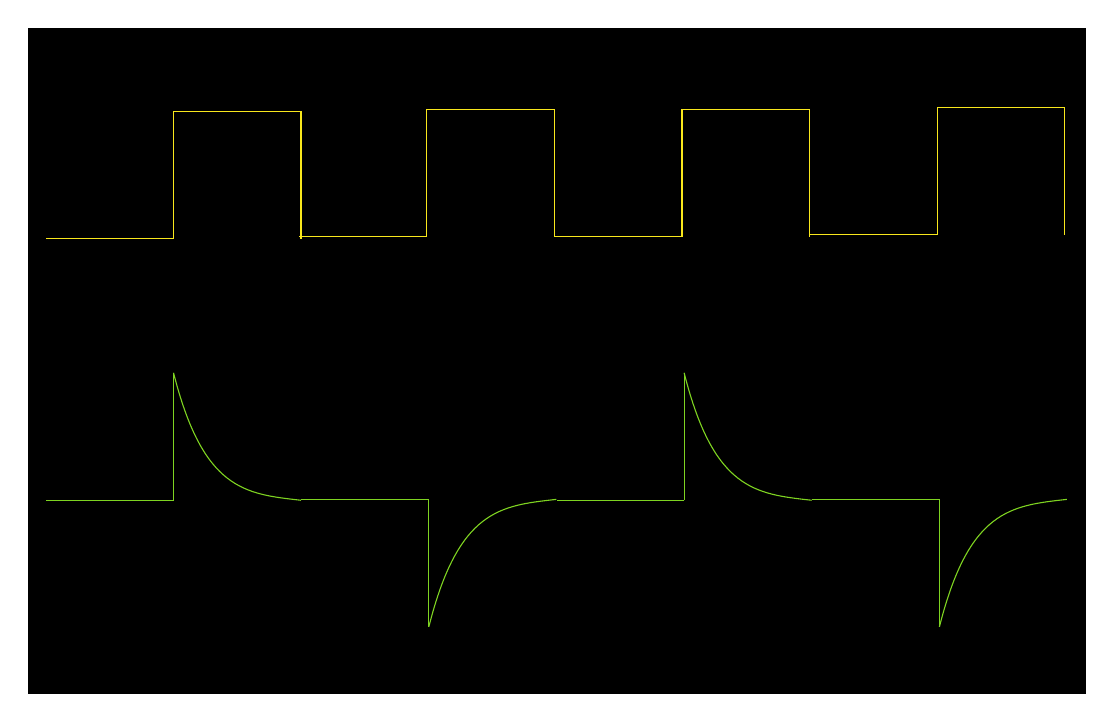
\begin{tikzpicture}[x=0.75pt,y=0.75pt,yscale=-1,xscale=1]
%uncomment if require: \path (0,416); %set diagram left start at 0, and has height of 416

%Shape: Rectangle [id:dp5316083172836576] 
\draw  [fill={rgb, 255:red, 0; green, 0; blue, 0 }  ,fill opacity=1 ] (74.71,62.58) -- (584,62.58) -- (584,383) -- (74.71,383) -- cycle ;
%Straight Lines [id:da8192848431655619] 
\draw [color={rgb, 255:red, 248; green, 231; blue, 28 }  ,draw opacity=1 ]   (389.71,163) -- (328.29,163) ;
%Straight Lines [id:da746913960603264] 
\draw [color={rgb, 255:red, 248; green, 231; blue, 28 }  ,draw opacity=1 ]   (389.71,163) -- (389.71,101.58) ;
%Straight Lines [id:da5827505568276088] 
\draw [color={rgb, 255:red, 248; green, 231; blue, 28 }  ,draw opacity=1 ]   (451.13,101.58) -- (389.71,101.58) ;
%Straight Lines [id:da41717341580276823] 
\draw [color={rgb, 255:red, 248; green, 231; blue, 28 }  ,draw opacity=1 ]   (451.13,163) -- (451.13,101.58) ;
%Straight Lines [id:da47673434295574824] 
\draw [color={rgb, 255:red, 248; green, 231; blue, 28 }  ,draw opacity=1 ]   (512.71,162) -- (451.29,162) ;
%Straight Lines [id:da7741255568939518] 
\draw [color={rgb, 255:red, 248; green, 231; blue, 28 }  ,draw opacity=1 ]   (512.71,162) -- (512.71,100.58) ;
%Straight Lines [id:da9520384444017516] 
\draw [color={rgb, 255:red, 248; green, 231; blue, 28 }  ,draw opacity=1 ]   (574.13,100.58) -- (512.71,100.58) ;
%Straight Lines [id:da7581455667970272] 
\draw [color={rgb, 255:red, 248; green, 231; blue, 28 }  ,draw opacity=1 ]   (574.13,162) -- (574.13,100.58) ;
%Straight Lines [id:da10714401805452489] 
\draw [color={rgb, 255:red, 126; green, 211; blue, 33 }  ,draw opacity=1 ]   (144.71,290) -- (83.29,290) ;
%Straight Lines [id:da016366227196888294] 
\draw [color={rgb, 255:red, 126; green, 211; blue, 33 }  ,draw opacity=1 ]   (144.71,290) -- (144.71,228.58) ;
%Curve Lines [id:da19521770808480476] 
\draw [color={rgb, 255:red, 126; green, 211; blue, 33 }  ,draw opacity=1 ]   (144.71,228.58) .. controls (159,285) and (179,287) .. (206.13,290) ;
%Straight Lines [id:da5968254583298855] 
\draw [color={rgb, 255:red, 126; green, 211; blue, 33 }  ,draw opacity=1 ]   (267.71,289.58) -- (206.29,289.58) ;
%Straight Lines [id:da2640603681382274] 
\draw [color={rgb, 255:red, 126; green, 211; blue, 33 }  ,draw opacity=1 ]   (267.71,289.58) -- (267.71,351) ;
%Curve Lines [id:da7436841005446766] 
\draw [color={rgb, 255:red, 126; green, 211; blue, 33 }  ,draw opacity=1 ]   (267.71,351) .. controls (282,294.58) and (302,292.58) .. (329.13,289.58) ;
%Straight Lines [id:da7745367566587171] 
\draw [color={rgb, 255:red, 248; green, 231; blue, 28 }  ,draw opacity=1 ]   (144.71,164) -- (83.29,164) ;
%Straight Lines [id:da9883928919106464] 
\draw [color={rgb, 255:red, 248; green, 231; blue, 28 }  ,draw opacity=1 ]   (144.71,164) -- (144.71,102.58) ;
%Straight Lines [id:da9610397579562393] 
\draw [color={rgb, 255:red, 248; green, 231; blue, 28 }  ,draw opacity=1 ]   (206.13,102.58) -- (144.71,102.58) ;
%Straight Lines [id:da39587765110238093] 
\draw [color={rgb, 255:red, 248; green, 231; blue, 28 }  ,draw opacity=1 ]   (206.13,164) -- (206.13,102.58) ;
%Straight Lines [id:da3870937751022798] 
\draw [color={rgb, 255:red, 248; green, 231; blue, 28 }  ,draw opacity=1 ]   (266.71,163) -- (205.29,163) ;
%Straight Lines [id:da8718291341512958] 
\draw [color={rgb, 255:red, 248; green, 231; blue, 28 }  ,draw opacity=1 ]   (266.71,163) -- (266.71,101.58) ;
%Straight Lines [id:da9666508787169255] 
\draw [color={rgb, 255:red, 248; green, 231; blue, 28 }  ,draw opacity=1 ]   (328.13,101.58) -- (266.71,101.58) ;
%Straight Lines [id:da626629296771257] 
\draw [color={rgb, 255:red, 248; green, 231; blue, 28 }  ,draw opacity=1 ]   (328.13,163) -- (328.13,101.58) ;
%Straight Lines [id:da27921367455211055] 
\draw [color={rgb, 255:red, 126; green, 211; blue, 33 }  ,draw opacity=1 ]   (390.71,290) -- (329.29,290) ;
%Straight Lines [id:da30490120179861413] 
\draw [color={rgb, 255:red, 126; green, 211; blue, 33 }  ,draw opacity=1 ]   (390.71,290) -- (390.71,228.58) ;
%Curve Lines [id:da4165120589677904] 
\draw [color={rgb, 255:red, 126; green, 211; blue, 33 }  ,draw opacity=1 ]   (390.71,228.58) .. controls (405,285) and (425,287) .. (452.13,290) ;
%Straight Lines [id:da22316385692079077] 
\draw [color={rgb, 255:red, 126; green, 211; blue, 33 }  ,draw opacity=1 ]   (513.71,289.58) -- (452.29,289.58) ;
%Straight Lines [id:da7163181178647944] 
\draw [color={rgb, 255:red, 126; green, 211; blue, 33 }  ,draw opacity=1 ]   (513.71,289.58) -- (513.71,351) ;
%Curve Lines [id:da46891152406721703] 
\draw [color={rgb, 255:red, 126; green, 211; blue, 33 }  ,draw opacity=1 ]   (513.71,351) .. controls (528,294.58) and (548,292.58) .. (575.13,289.58) ;





\end{tikzpicture}

    \caption{Input Wave (Top) and Output Wave (Bottom) Approximation}
    \label{fig:2}
  \end{figure}

  \subsection{Q6} As the frequency increases, the capacitor is unable to discharge quick enough, so the output begins to look more and more like a square wave.

\section{Conclusion}

Overall, this laboratory experiment introduced us to the concept of physical active filters through transform and Fourier analysis. Furthermore, this time the operational amplifier was a real-world circuit component, making it easier to grasp the concept.

\end{document}
